\subsection{Simulation Setup for Combined Yaw and Thrust Control} \label{WakeModel} 
As before, WFSim is used to obtain open-loop data and for closed-loop controller testing. This section provides an overview of the WFSim environment and describes the specific test cases utilized for Koopman system identification in this context.

Figure~\ref{fig:BlockDiagramFarm} illustrates the underlying concept for the WRC-AIC strategies applied to the two-turbine wind farm. Note that the primary difference from the setup in Section~\ref{sec:AdaptiveWindFarmqLMPCforAIC} is that the yaw control signal of the upstream turbine WT1, $\gamma_1$, is now an active control variable.

\begin{figure}[h]
    \centering
    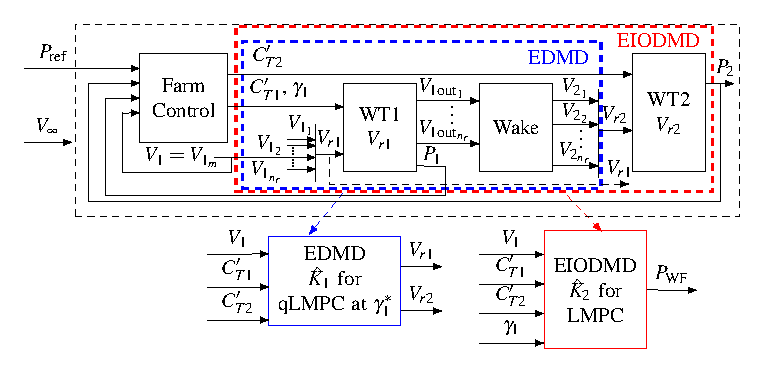
\includegraphics[width=0.9\textwidth]{figures/figuresBlockDiagram_IFAC23/farmCtrl17_P_multVthesis_WRCAIC_EIODMD.pdf}
    \caption[Block diagram of WFSim for WRC-AIC]{Block diagram of WFSim for WRC-AIC with farm control inputs $P_{\text{ref}}$, $P_1$, $P_2$, and $V_1 = V_{1_m}$, control signals $C_{T1}^{\prime}$, $C_{T2}^{\prime}$, $\gamma_1$, and freestream wind $V_\infty$. Local wind speeds upwind and downwind of WT1 are $V_{1_1} \dots V_{1_{n_r}}$ and $V_{1\text{out}_1} \dots V_{1\text{out}_{n_r}}$. Wind speeds upwind of WT2 are $V_{2_1} \dots V_{2_{n_r}}$. The input to the EDMD model (blue) are $V_1, C_{T1}^{\prime}, C_{T2}^{\prime}$ with effective wind outputs $V_{r1}, V_{r2}$. The input to the EIODMD model (red) are $V_1, C_{T1}^{\prime}, C_{T2}^{\prime}, \gamma_1$ with farm power output $P_{\text{WF}} = P_1 + P_2$.}
    \label{fig:BlockDiagramFarm}
\end{figure}

The signals are defined as in previous sections, with the exceptions that the freestream wind speed is kept constant and $\gamma_1$ is commanded by the farm controller. This results in the following signal configuration:
\begin{description}
    \item[-] The freestream wind $V_\infty$ is constant at $8$\,m/s and aligned perpendicular to the turbines for all simulations in this section.
    \item[-] The farm power reference $P_{\text{ref}}$.
    \item[-] The measured wind $V_1$ at WT1, used as a controller input as established in Section~\ref{sec:AdaptiveWindFarmqLMPCforAIC} and the underlying study~\cite{dittmer2022data}.
    \item[-] The thrust control signal $C_{T1}^{\prime}$ and yaw $\gamma_1$ of WT1, with the latter being a variable here, while it was fixed at $0$\,deg in Section~\ref{sec:AdaptiveWindFarmqLMPCforAIC}.
    \item[-] The effective wind speed $V_{r1}$ (mean wind speed over the rotor disk) and power $P_1$ of WT1.
    \item[-] Corresponding input and output signals for turbine WT2.
\end{description}
The farm layout and turbine parameters follow Table~\ref{table:WfSim}. For EDMD, estimates $\Tilde{U}_{ri}$ are calculated from $P_i$ assuming a known power coefficient $c_p$.

Previous publications utilizing WFSim~\cite{boersma2017tutorial,doekemeijer2018online, sharan2022Koopman, dittmer2022data} focused on thrust control $C_T^{\prime}$ for AIC, resulting in $n_u = n_{\text{WT}}$ control inputs. However, WFSim also supports yaw control $\gamma$ for wake redirection. In a two-turbine scenario, this could result in $2n_{\text{WT}}$ inputs; however, for this proof of concept, only the yaw of the first turbine is varied. Since the second turbine has no downstream neighbors, its optimal orientation remains $\gamma_2 = 0$\textdegree{}, resulting in $n_u = 3$ control inputs for this study.

Open-loop data is acquired from a WFSim simulation of $n_o = 28000$ samples, where one sample $k$ corresponds to $1$\,s. The thrust signals $C_{T1}^{\prime}$ and $C_{T2}^{\prime}$ are constructed from white noise (mean 1.7, variance 0.3, lower and upper limits 0.1 and 2.0, respectively) held constant for $5$\,samples. The yaw signal $\gamma_1$ is stepped by $5$\textdegree{} every $4000$\,samples from $0$\textdegree{} to $30$\textdegree{} and augmented with zero-mean band-limited noise (variance $0.5$\textdegree{}). These signals ensure data excitation across all relevant frequencies and control input combinations.

The matrices $\bm{X}_{\text{EIODMD}}$ and $\bm{X}_{\text{EIODMD},+}$ are constructed from input, state and output samples:
\begin{equation}
    \bm{w}(k) = \begin{bmatrix} C_{T1}'(k) \quad C_{T2}'(k) \quad \gamma_1(k) \end{bmatrix}^T, \quad \bm{x} = [V_{r1} \;\; V_{r2}]^T,  \quad 
    \bm{y}(k) = P_{\text{WF}}(k).
\end{equation}
and are assembled by stacking snapshots as follows:
\begin{align}
    \bm{X}_{\text{EIODMD}} &= \bigl[ [\bm{x}(k)^T \quad \bm{w}(k)^T]^T \bigr]_{k=1}^{n_o-1}, \\
    \bm{X}_{\text{EIODMD},+} &= \bigl[ [\bm{x}(k+1)^T \quad \bm{y}(k)^T]^T \bigr]_{k=1}^{n_o-1},
\end{align}

These matrices are used to construct two Koopman matrices, $\hat{K}_1$ (EDMD) and $\hat{K}_2$ (EIODMD), for the respective MPC designs. The system dynamics are of $6^{\text{th}}$ order with:
\begin{description}
    \item[-] Lifted states $\bm{\varphi} = [\bm{x}^T \;\; (\bm{x}^2)^T \;\; (\bm{x}^3)^T]^T$. The quadratic and cubic terms reflect the relationship between wind, force and power.
    \item[-] Inputs $w_{K1} = [C_{T1} \;\; C_{T2} \;\; V_1]^T$ and $w_{K2} = [C_{T1} \;\; C_{T2}'\;\; V_1\;\; \gamma_1]^T$.
    \item[-] EDMD outputs $\bm{y}_{K1} = [V_{r1} \;\; V_{r2}]^T$ and EIODMD outputs $\bm{y}_{K2} = P_{\text{WF}}$.
\end{description}

The matrix $\hat{K}_{w2} \in \mathbb{R}^{7\times11}$ is reordered to separate the contributions of the system states via the matrices $A_w \in \mathbb{R}^{6\times6}$ and $C_w \in \mathbb{R}^{1\times6}$, control inputs via $B_u \in \mathbb{R}^{6\times3}$ and $D_u \in \mathbb{R}^{1\times3}$, and the measured disturbance input $V_1$ via $B_d \in \mathbb{R}^{6\times1}$ and $D_d \in \mathbb{R}^{1\times1}$. To account for the disturbance as a state in the linear MPC, the matrices are augmented, resulting in the state-space matrices $A_{\hat{K}2} \in \mathbb{R}^{7\times7}$, $B_{\hat{K}2} \in \mathbb{R}^{7\times3}$, $C_{\hat{K}2} \in \mathbb{R}^{1\times7}$, and $D_{\hat{K}2} \in \mathbb{R}^{1\times3}$. The relationship to the original matrices obtained from EIODMD is given by:

\begin{align*} 
    \hat{K}_{w2} = \left[\begin{array}{c|cc} 
        A_w & B_d & B_u\\ 
        \hline 
        C_w & D_d & D_u 
    \end{array}\right] \implies
    \hat{K}_{2} = \left[\begin{array}{cc|c} 
        A_w & B_d & B_u\\ 
        \bm{0}_{1\times6} & 1 & \bm{0}_{1\times3}\\
        \hline 
        C_w & D_d & D_u 
    \end{array}\right].
\end{align*}

The specific formulation and implementation of the qLMPC (based on $\hat{K}_1$) and linear Koopman MPC (based on $\hat{K}_2$) are detailed in Section~\ref{qLMPCDesign}.